\documentclass{article}
\usepackage{enumitem}
\usepackage{hyperref}

\usepackage{rotating}

\usepackage{listings}
\begin{document}

\begin{figure}[t]
\centering
	
\includegraphics[height=6.25cm,keepaspectratio]{Figures/logo}
\end{figure}

\title{TrackMe \\ Software Engineering 2 Project\\ \textit{ATD Document} }
\author{Stefano Martina, Alessandro Nichelini, Francesco Peressini
		\\ \\ A.Y. 2018/2019 \\ Version 1.0.0}
		
\maketitle
\newpage

\tableofcontents
\newpage

\section{Introduction}

\subsection{Purpose and Scope} 
The Acceptance Test Document has the purpose of evaluating the adherence of the implementation with respect to the  documents previously delivered. \newline
To do so, we have considered the three documents available in the provided GitHub repository.

\subsection{Reference} 
	As said above, the three documents analysed are:
	\begin{itemize}
		\item \textbf{ITD Document (v.1.0)}: \href{https://github.com/danmontesi/FossatiMontesiSgherzi/blob/master/delivery/ITD.pdf}{link}
		\item \textbf{DD Document (v.1.1)}: \href{https://github.com/danmontesi/FossatiMontesiSgherzi/blob/master/delivery/DD2.pdf}{link} 
		\item \textbf{RASD Document (v.1.2)}: \href{https://github.com/danmontesi/FossatiMontesiSgherzi/blob/master/delivery/RASD3.pdf}{link}
	\end{itemize}
	
\subsection{Overview} 
The document is organised in this way:
\begin{itemize}
	\item \textbf{Project}: the identification of the project we have analysed;
	\item \textbf{Installation Setup}: explains what we did to install the prototype of the tested project as well as any problem or incoherency we have found following the provided documentation;
	\item \textbf{Acceptance Tests}: the acceptance test cases we have applied and the corresponding outcome.
\end{itemize}

\subsection{Revision History}
\begin{itemize}
	\item 1.0.0 - Initial version (20/01/2019)
\end{itemize}

\newpage
\section{Project}
\subsection{Project info}
In this section we present the details about the project we have tested.
\subsubsection{Authors}
\begin{itemize}
	\item Daniele Montesi - 912980
	\item Nicola Fossati - 915244
	\item Francesco Sgherzi - 915377
\end{itemize}

\subsubsection{Links}
\begin{itemize}
	\item \textbf{GitHub repository}: \href{https://github.com/danmontesi/FossatiMontesiSgherzi}{link}
\end{itemize}

\newpage
\section{Installation Setup}
\subsection{Backend }
\subsubsection{Installation and launch}
	We have installed the backend as explained in the ITD Document, with the only exception of the particular system-dependent command (we tested the project on macOS).\newline
	We installed the following module with \textit{"brew"} command:
	
	\begin{itemize}
		\item \textbf{PostgreSQL}: an open source object-relational database system;
		\begin{itemize}
			\item	installed with the command: \textit{brew install postgresql}
		\end{itemize}
		\item \textbf{NodeJS}: an asynchronous event driven JavaScript runtime.
		\begin{itemize}
			\item	installed with the command: \textit{brew install nodejs}
		\end{itemize}
	\end{itemize}
	
	After the launch of the postgre service (with the command \textit{brew services start postgresql}), we created a new database and a new role for the admin user. \newline
	Then, with the new role just created, we imported the dump of the database provided in the Implementation folder of the previously mentioned repository.
	As last step we have configured the \textit{"start.sh"} file with the following configuration and launched it with the command \textit{"node app.js"}.
	\begin{figure}[h!]
		\centering
		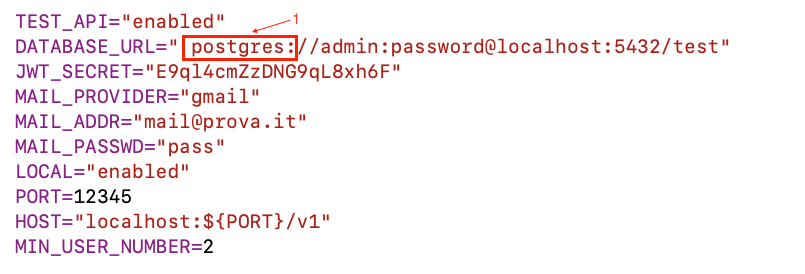
\includegraphics[height=4.25cm,keepaspectratio]{Figures/error1}
		\caption{Error in the database configuration}
	\end{figure}
	
\subsubsection{Conclusion}
We didn't encounter particular issues, the guide lines are clear and enough explicative.\newline
The only thing which makes sense to be mentioned is one error encountered during the database connection. It always responds with "\textit{message: role //password// does not exist}". This is due to a small error in the configuration file, probably to the fact that is a machine dependant parameter (view image 1).

\newpage	
\subsection{Frontend}
\subsubsection{Installation and launch}
Regarding the Android mobile application, we have installed the provided APK file on an Android Smartphone. We also tried to install it on a few simulators.\newline
\\For what concerns the iOS app, we managed to install Flutter SDK and to build the application, however we would have preferred to have a more precise and coincise guide in the ITD document such the one provided for the Android environment. \newline
\\Lastly, regarding the web-app, we launched it using the command\\ \textit{"python3 -m http.server"}, as explained in the guidelines.

\subsubsection{Conclusion}
Following the instructions on the ITD Document, on an Android smartphone everything works correctly.
Doing the same steps on a simulator, the application crashes, probably due to some incompatibilities with the running version of the simulator itself.	\newline
\\iOS app correctly built and run on simulator.\newline
\\The web-app works correctly.

\newpage
\section{Acceptance Tests}
\subsection{Tests}

For the acceptance tests, we worked on the mobile Android application but the results can be considered valid also for the iOS application  since, as explained  in RASD and DD documents, both the applications share the same codebase. Moreover, the tested project doesn't use platform-dependent frameworks or technologies (with the exception of the Google Maps framework that has been reported as a known issue); all the results are actually valid for both platforms.\\\\
We proceeded testing each requirement that has been declared as "implemented" in the ITD document.

\subsection{Actor registration}
\begin{itemize}
	\item {[RM$_M$]}: \textit{OK.} Users can register providing information required, but registration process succeed also without an associated smartwatch.
	\item {[R2$_M$]}: \textit{OK.} Implementation works: registration process is successful if  there is NOT another user with the same email/fiscal code. However, errors-handling is not able to distinguish between a duplicate email or a duplicate fiscal code.
	\item {[R11$_W$]}: \textit{OK.} Organisers can successfully register.
	\item {[R1$_W$]}: \textit{OK.} Companies can successfully register.
	\item {[R14$_C$]}: \textit{OK.} Information such as birthday and fiscal code are validated through UI form.
\end{itemize}

\subsection{Actor Authentication} 
\begin{itemize}
	\item {[R1$_M$]}: \textit{OK.} Users can successfully log into the application.
	\item {[R12$_M$]}: \textit{OK.} Organisers can successfully log into the application.
	\item {[R2$_W$]}: \textit{OK.} Companies  can successfully log into the application.
\end{itemize}

\subsection{Individuals Management}
\begin{itemize}
	\item {[R6$_M$]}: \textit{OK.} Requests appear in the right section of the mobile app. Users can actually accept or decline them.
	\item {[R2$_C$]}: \textit{OK.} Users received notification about new requests at the email address provided during the registration phase.
\end{itemize}

\subsection{Data management}
\begin{itemize}
	\item {[R4$_C$]}: \textit{OK.} We can't directly test this feature, but it seems that all data loaded into the application is also available after a logout.
	\item {[R5$_C$]}: \textit{OK.} Same as the previous one.
	\item {[R2$_S$]}: \textit{OK.} Assuming the requirement {[R2$_S$]} as \textit{"App can send data registered locally to Data4Help Web App"}, the mobile application can actually send data to the Web App.
\end{itemize}

\subsection{Query management}

\begin{itemize}
	\item {[R6$_W$]}: \textit{OK.} Logged-in companies can actually query on some group of individuals data providing location, heart rate and accelerometer information.
	\item {[R7$_W$]}: \textit{OK.} Companies can actually request data of individuals. 
	\item {[R8$_W$]}: \textit{OK.} Companies can access to individuals data through the web app.
	\item {[R9$_W$]}: \textit{OK.} The web app actually provides the data download functionality.
	\item {[R6$_C$]}: \textit{OK.} After the acceptance by the user, third parties can retrieve data from the individual correctly. 
	\item {[R6bis$_W$]}: \textit{OK.} The web app implement the subscription functionality through a slider. The company actually receives a notification when new data is available.
	\item {[R7$_C$]}: \textit{KO.} Check the "Issues" section.
\end{itemize}

\subsubsection{Issues}
During the testing of requirements {[R7$_W$]} and {[R8$_W$]}, we have found the following issue:
\begin{itemize}
	\item the process fails if requests are made by a company that has the same email address of a user. \\The error message is the following: \textit{"Error: Unauthorised. Retry"} and it appears on the website as an alert. However, since it's unlikely that a company uses the same address of a user, we still marked the requirement as "OK".
\end{itemize}

\subsection{Race management}
\begin{itemize}
	\item {[R8$_M$]}: \textit{OK.} Registration is possible through the track4run tab at anytime.
	\item {[R9$_M$]}: \textit{KO.} Check the "Issues" section.
	\item {[R13$_M$]}: \textit{OK.} Organisers actually have all the necessary information to create a path.
	\item {[R14$_M$]}: \textit{OK.} Organisers can define the path of the run and the starting/ending time and date.
\end{itemize}

\subsubsection{Issues}
Concerning requirement {[R9$_M$]}, the application only displays the name of the run, its status and (partially) the position of participants. Information about the starting point, the ending point, the precise path and the run length are not available.

\subsection{Users Spectating Race}
\begin{itemize}
	\item {[R10$_M$]}: \textit{KO.} Check the "Issues" section.
	\item {[R13$_C$]}: \textit{KO.} Check the "Issues" section.
\end{itemize}

\subsubsection{Issues}
Concerning the requirements {[R10$_M$]} and {[R13$_C$]}, the application only displays a static pin on a Google Maps interface for each participants of the run. \\ We were not able to test if the application actually track the position of the runners, also considering that the authorisation to access to the actual location of the runners were never asked at no time.

\newpage
\section{Conclusion}
Apart from the few issues described above and in the ITD document provided to us by the developers, the application is working as expected: all the major features described by the ITD document are present and ready to be used by a final user. \\\\
The user interface is pretty intuitive and easy to user, even at a first start; the initial set-up is super easy concerning the installation of the application for Android, a little bit difficult concerning the installation on an iOS device, also due to the strictly policy imposed by Apple. \\\\
Future update should focus on providing new features to the final user such as AutomatedSOS, for which is already present a section in the application.

\newpage
\section{Effort spent}
\begin{itemize}
	\item Stefano Martina: 5.00h
	\item Alessandro Nichelini: 5.00h
	\item Francesco Peressini: 5.00h
\end{itemize}

\end{document}